\documentclass[10pt,a4paper]{article}

% --- Encoding, Fonts & Microtypography ---
\usepackage[utf8]{inputenc}
\usepackage[T1]{fontenc}
\usepackage{lmodern}
\usepackage{microtype}
\usepackage{comment}
\usepackage{booktabs} % Required for \toprule, \midrule, \bottomrule
\usepackage{makecell} % Required for multi-line cells with \makecell
\usepackage{caption}  % Recommended for table captions
\usepackage{float}
\usepackage{wrapfig} 
\usepackage{comment} %for multiline comments
% --- Page Layout ---
\usepackage{geometry}
\geometry{a4paper, margin=1in}

% --- Graphics & Figures ---
\usepackage{graphicx}
\usepackage{subcaption}
% Set the default folder for images/graphs.
\graphicspath{{graphs/}}

% --- Hyperlinks ---
\usepackage{hyperref}
\hypersetup{
    colorlinks=true,
    linkcolor=black,
    urlcolor=blue,
    citecolor=black
}

% --- Bibliography with BibLaTeX ---
\usepackage{biblatex}
\addbibresource{bib.bib}
\usepackage{appendix}


\title{Group M MiniTwit Report \\ DevOps Spring 2025 KSDSESM1KU}
\author{Iulia Maria Negrila, Max Bezemer, Olivia Burca, Tore Kjelds, Su Mei Gwen Ho \\ iune@itu.dk, mbez@itu.dk, olbu@itu.dk, tokj@itu.dk, suho@itu.dk}
\date{\today}

\begin{document}

\maketitle
\tableofcontents
\newpage
\section{Introduction}
%iulia&olivia
%mini overview of project here.
This report documents the design, implementation, and evolution of our ITU-MiniTwit system throughout the DevOps course. Working as a team, we began with a basic Python-based "Twitter clone" and migrated it to a Go-based architecture, applying DevOps principles at every stage. Over the semester, we incrementally integrated tools and practices such as containerization, infrastructure as code, continuous integration and deployment, monitoring, logging, and scaling strategies. This report outlines the technical decisions we made, the tools and workflows we adopted, and the lessons learned while building a reliable, testable, and maintainable system.

\section{System}
%This sections concerns the design of our MiniTwit system. Wherein we describe and discuss the design and architecture of the system. Following that a reflection of the different tools and dependencies used for the project. Finally we assess the current state of the system, using INSERT PERFORMANCE METRIC.
%MSc students should argue for the choice of technologies and decisions for at least all cases for which we asked you to do so in the tasks at the end of each session.

\subsection{Design \& Architecture}
%Our Minitwit system evolved during the course into the current architecture shown in Fig. \ref{fig:Deployment}. It features a web interface that communicates with a backend API; the API reads and writes to a database. To enhance availability and reduce downtime, the system is deployed using a hot–cold server configuration, facilitated through \textbf{keepalived}. This setup ensures that a backup instance can be quickly activated if the primary server (Droplet) fails. The entire system is hosted on DigitalOcean, where we also utilize a PostgreSQL database to manage persistent data storage. In addition to its core functionality, the system includes support for both monitoring and logging, which are discussed in more detail in Sections \ref{sec:monitoring} and \ref{sec:logging}. 

Our Minitwit system evolved during the course into the current architecture shown in Fig. \ref{fig:Deployment}. The entire system is hosted on DigitalOcean, where a web interface communicates with a backend API; the API reads and writes to a PostgreSQL database where persistent data is managed. In addition both monitoring and logging are integrated, including volumes to store logs and metrics. Fig. \ref{fig:Deployment} shows how the servers (Droplets) are set up; each runs eight containers when active as well as a Keepalived daemon for the failover mechanism. At all times one server is active, serving the Minitwit web application and accessing the database. To ensure availability floating IPs are used to point to the appropriate server during failures and updates. All features mentioned here are expanded upon in coming sections.

\begin{figure}[!htb]
    \centering
    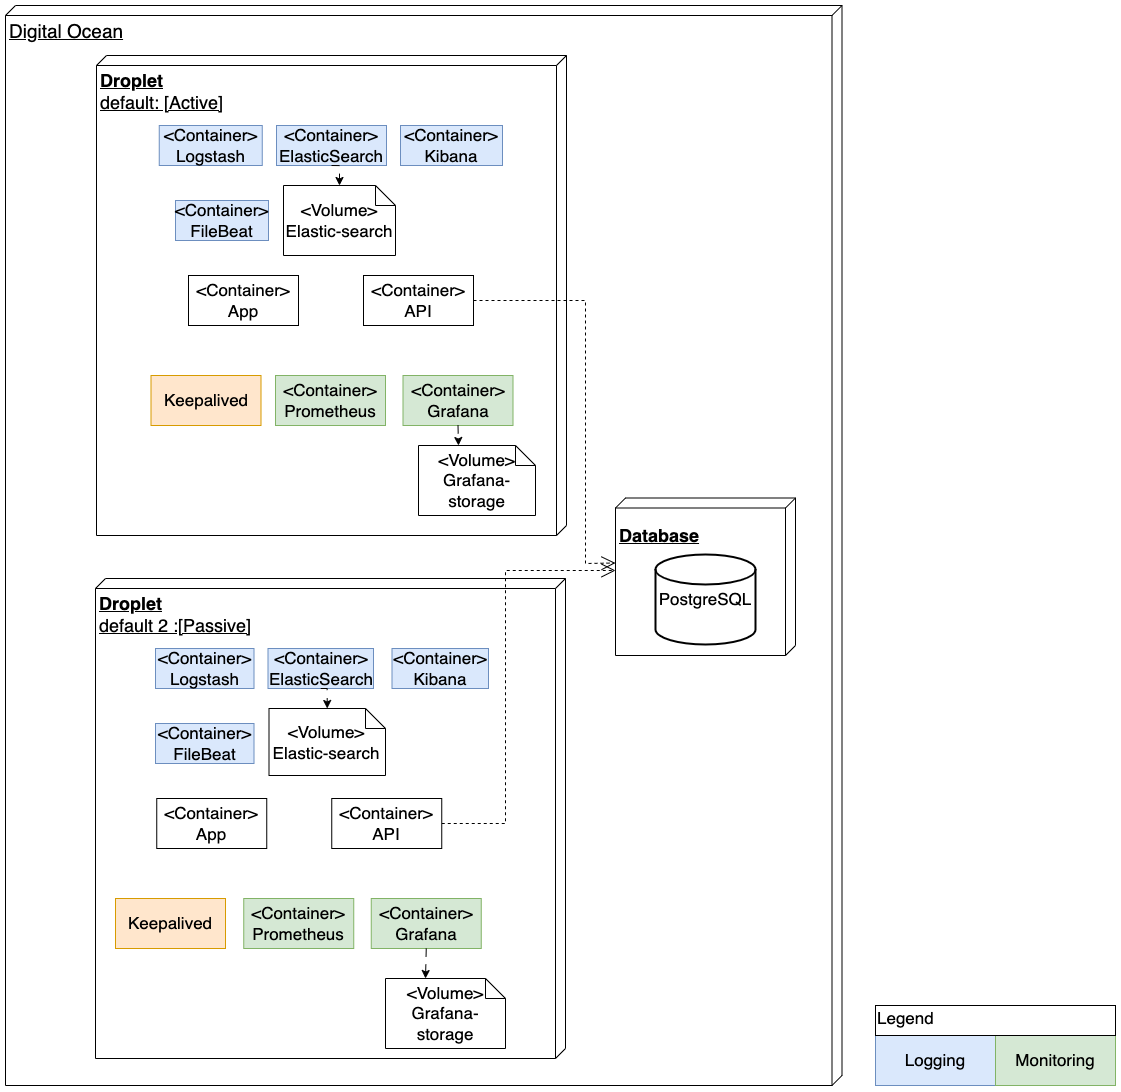
\includegraphics[width=0.9\linewidth]{Images/Deployment_diagram-Newer.drawio.png}
    \caption{Deployment diagram}
    \label{fig:Deployment}
\end{figure}

%gwen&tore
%static view
%- overall abstract system diagram DONE
%- UML deployment diagram (incl load-balancing)

\subsection{Dependencies \& Tools}
%iulia&olivia
%All dependencies of your ITU-MiniTwit systems on all levels of abstraction and development stages. That is, list and briefly describe all technologies and tools you applied and depend on.`

\subsubsection*{Development \& Runtime}
\begin{itemize}
  \item \textbf{Go (Golang)} – Primary language for the application. 
  \item \textbf{GORM} – ORM for Go used to interact with the database.
  \item \textbf{Gorilla Mux} – HTTP router and URL matcher for Go, used to handle routing in the backend API.
  \item \textbf{Python} – Used for testing, especially API and UI validation.
  \item \textbf{Docker \& Docker Compose} – Containerization of all services and orchestration for local and CI environments.
\end{itemize}

\subsubsection*{Infrastructure}
\begin{itemize}
  \item \textbf{Terraform} – Infrastructure as Code to provision and manage DigitalOcean droplets, floating IPs, and DigitalOcean Spaces.
  \item \textbf{DigitalOcean} – Cloud provider hosting the production infrastructure, including our high availability setup.
  \item \textbf{Vagrant} – Used initially to provision reproducible local development environments.
  \item \textbf{Keepalived} – Provides failover between active and standby droplets using floating IP reassignment.
  \item \textbf{Docker Hub} - Used to store the Docker images.
\end{itemize}

\subsubsection*{CI/CD \& Automation}
\begin{itemize}
  \item \textbf{GitHub Actions} – Automates testing, building, deploying, and releasing workflows.
  \item \textbf{gofmt} – Enforces Go code formatting standards.
  \item \textbf{golangci-lint} – Static analysis aggregator for Go code quality.
  \item \textbf{dockerfilelint} – Linter for validating Dockerfiles.
  \item \textbf{GitHub CLI} – Used for automated GitHub release creation. 
  \item \textbf{SonarQube} – Used to automatically analyze code quality.
\end{itemize}

\subsubsection*{Testing \& Validation}
\begin{itemize}
  \item \textbf{Go test} – For backend unit and integration tests.
  \item \textbf{pytest} – Runs API-level tests written in Python.
  \item \textbf{Selenium (with Firefox + Geckodriver)} – Powers UI and end-to-end testing in a headless browser.
  \item \textbf{unittest (Python)} – Traditional functional tests.
  \item \textbf{SQLite3} – Lightweight database used in testing environments to verify correctness.
\end{itemize}

\subsubsection*{Monitoring \& Logging}
\begin{itemize}
  \item \textbf{Prometheus} – Collects metrics from application containers, especially health and performance indicators.
  \item \textbf{Grafana} – Provides dashboards and visualizations of Prometheus metrics at \texttt{localhost:3000}.
  \item \textbf{Elasticsearch} – Central log storage and indexing engine for collecting application logs.
  \item \textbf{Logstash} – Processes and forwards logs from containers into Elasticsearch.
  \item \textbf{Filebeat} – Lightweight log shipper running on containers to collect logs.
  \item \textbf{Kibana} – UI for querying and visualizing logs from Elasticsearch (at \texttt{localhost:5601}).
  \item \textbf{Keepalived} – Also monitors app health to trigger failover, contributing indirectly to availability observability.
\end{itemize}

\subsection{Subsystems Interactions}
%gwen&tore
%dynamic view
We chose two common scenarios to illustrate a dynamic view of our system. First the sequence diagram below, Fig. \ref{fig:seq_user}, shows the flow of events triggered by a user when they attempt to send a new message. It starts with the User pressing submit, having filled out the HTML form which makes the app issue a POST request to the API. Upon receiving the request an initial logging event records the attempt. The API queries the PostgreSQL database to retrieve the User's ID which it then uses to create a new message entry. Once the message is successfully saved in the database, confirmation that the message was stored without error is logged and two separate counters used for system monitoring are updated. Finally, the API returns a 204 No Content HTTP status code to the Simulator to signal that the message was properly processed.

\begin{figure}[!htb]
    \centering
    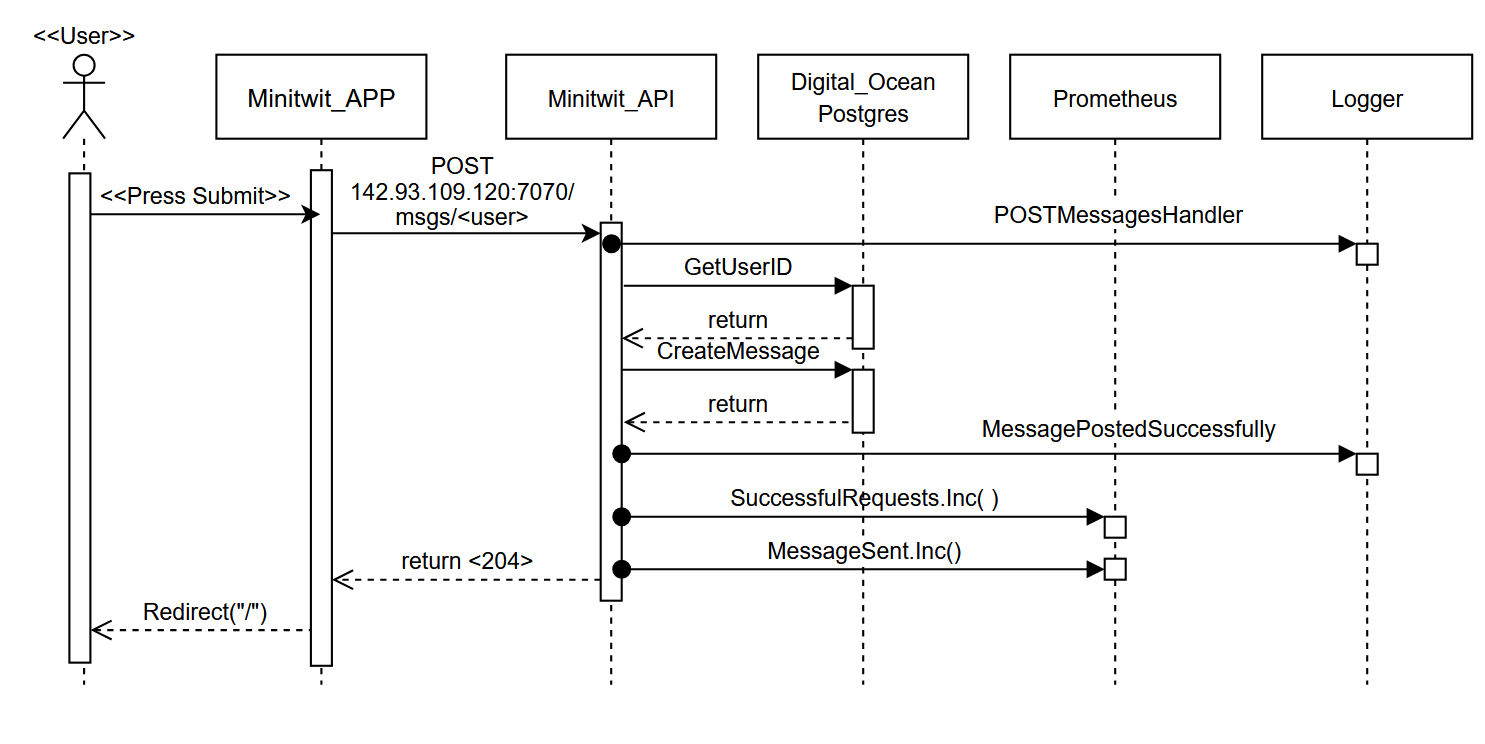
\includegraphics[width=0.9\linewidth]{Images/seq_user.png}
    \caption{Sequence diagram of a successful sent message from the user's perspective}
    \label{fig:seq_user}
\end{figure}

The next sequence diagram, Fig. \ref{fig:seq_fail}, shows a common interaction between the Simulator and our system this semester. When an error prevents a User from being created, the Simulator may later attempt to send a message through a \textbf{POST} request at the "\textit{/msgs/<<User>>}" endpoint. This is unsuccessful since the User does not exist and therefore cannot post.\\ \\ 

\begin{figure} [!htb]
    \centering
    \includegraphics[width=0.9\linewidth]{Images/Seq_fail.png}
    \caption{Sequence diagram of the Simulator trying to post a message as a non-existent user.}
    \label{fig:seq_fail}
\end{figure}
\newpage
\subsection{Current State}
%MAX
%Describe the current state of your systems, for example using results of static analysis and quality assessments.
We have been using SonarCloud since March 28 to monitor code quality. The Quality Gate passes, but deeper analysis highlights several areas for improvement:

\begin{itemize}
    \item \textbf{Code Duplication:} Currently at 4.4\%, exceeding the 3\% recommended threshold. New code remains within limits, but duplication is mainly due to repeated literals and logic across components.
    
    \item \textbf{Maintainability:} 55 open code smells, many flagged as high severity. These are mostly related to repeated strings that should be refactored into constants.
    
    \item \textbf{Reliability:} 10 minor issues, no blockers.
    
    \item \textbf{Security:} No active vulnerabilities, but 21 security hotspots, mostly due to hardcoded credentials in test files (e.g., \texttt{pwd = "super\_safe"}). These should not impact production and should be reviewed.
\end{itemize}

Summarising the above, the overall maintainability and reliability ratings sit at A, while the security rating is E. Technical debt is estimated at 6.5 hours. The codebase is in stable condition, but is in need of some maintenance to improve long-term quality.





%\clearpage
\section{Process}
\subsection{Continuous Integration and Deployment (CI/CD)}
%olivia
%A complete description of stages and tools included in the CI/CD chains, including deployment and release of your systems.
%create a diagram!
To automate building, testing and releasing our ITU-MiniTwit system, we implemented a CI/CD pipeline using GitHub Actions. We chose GitHub Actions due to its native integration with our GitHub-hosted repository, ease of configuration, and support for open-source projects. This allowed us to set up an effective pipeline without maintaining external CI infrastructure, which aligned well with the size and scope of our team project.

\subsubsection*{Pipeline Overview}

Our pipeline is triggered on every push to the \texttt{main} branch and consists of three main stages: \textbf{build}, \textbf{test}, and \textbf{deploy}.

\begin{enumerate}
\item
\subsubsection*{Build Stage}
\begin{itemize}
  \item The pipeline checks out the code and logs into Docker Hub using secrets stored securely in GitHub.
  \item It then builds two Docker images:
    \begin{itemize}
      \item \texttt{devoops-app} (the frontend)
      \item \texttt{devoops-api} (the backend)
    \end{itemize}
  \item These images are tagged and pushed to Docker Hub, using cache layers for efficiency.
\end{itemize}

\item
\subsubsection*{Test Stage}
\begin{itemize}
  \item After successful builds, the pipeline spins up a full test stack using 
  \texttt{docker-compose\_test\_local.yml} which runs containerized tests.
  \item This includes integration, API, UI, and end-to-end tests. The pipeline will fail fast if any test fails, stopping the deployment stage to ensure only verified code is released.
\end{itemize}

\item
\subsubsection*{Deploy Stage}
\begin{itemize}
  \item This stage involves deploying to our remote infrastructure on DigitalOcean using a \texttt{blue-green deployment strategy} based on two floating IPs. The full upgrade logic and IP switching process is described separately in the Upgrade Strategy section.
  \item A step using \texttt{terraform init} is also executed to set up the infrastructure. While this ensures the environment is up-to-date, we acknowledge that re-running \texttt{terraform init} and \texttt{apply} on every push may be excessive and could be optimized to only run when infrastructure-related files change.
\end{itemize}
\end{enumerate}

\subsubsection*{Static Analysis \& Quality Gates}

We integrated multiple static analysis tools as quality gates into a pipeline that runs when a pull request is created, to catch code issues early and enforce consistent formatting and linting:
\begin{itemize}
  \item \texttt{gofmt} checks Go code formatting.
  \item \texttt{golangci-lint} performs static analysis on Go files.
  \item \texttt{dockerfilelint} validates all Dockerfiles.
\end{itemize}

\subsubsection*{Release Automation}

We automated our release process using a GitHub Actions workflow that triggers on tags matching \texttt{v*}, creating versioned GitHub Releases with auto-generated notes. This ensures consistent, traceable production releases aligned with our deployment flow.

\subsection{Monitoring}
\label{sec:monitoring}
We use Prometheus and Grafana to monitor our system’s health. Metrics are instrumented with the Prometheus Go client library, registered via the default Prometheus registry, and exposed through the \textit{metrics} endpoint for Prometheus to scrape. \\ \\ 
For visualization we use Grafana, that uses prometheus as a data source and enables us to create and customize panels that visualizes the different metrics. \\\\ 
In relation to the James Turnbull monitoring maturity model\cite{turnbull2015monitoring}, ours would be considered reactive as we track specific errors in relation to specific endpoints and overall availability.\\\\
We do not do any front-end monitoring, as the course was primarily focused on the simulations interaction with our API.
\subsubsection{Metrics monitored}
We defined the following endpoints. Some, like \textit{Successful requests} track multiple endpoints and aggregate them in single time line for easier viewing and a reduction in overall panels in Grafana. The full dashboard can be seen in figure \ref{fig:dashboard}
\begin{itemize}
    \item \textbf{Uptime}
    \item \textbf{Successful requests (Tracks multiple endpoints)}
    \item \textbf{Unsuccessful requests (Tracks multiple endpoints)}
    \item \textbf{Follows}
    \item \textbf{Unfollows}
    \item \textbf{Successful messages sent}
    \item \textbf{Users not found}
\end{itemize}

\begin{figure} [!htb]
    \centering
    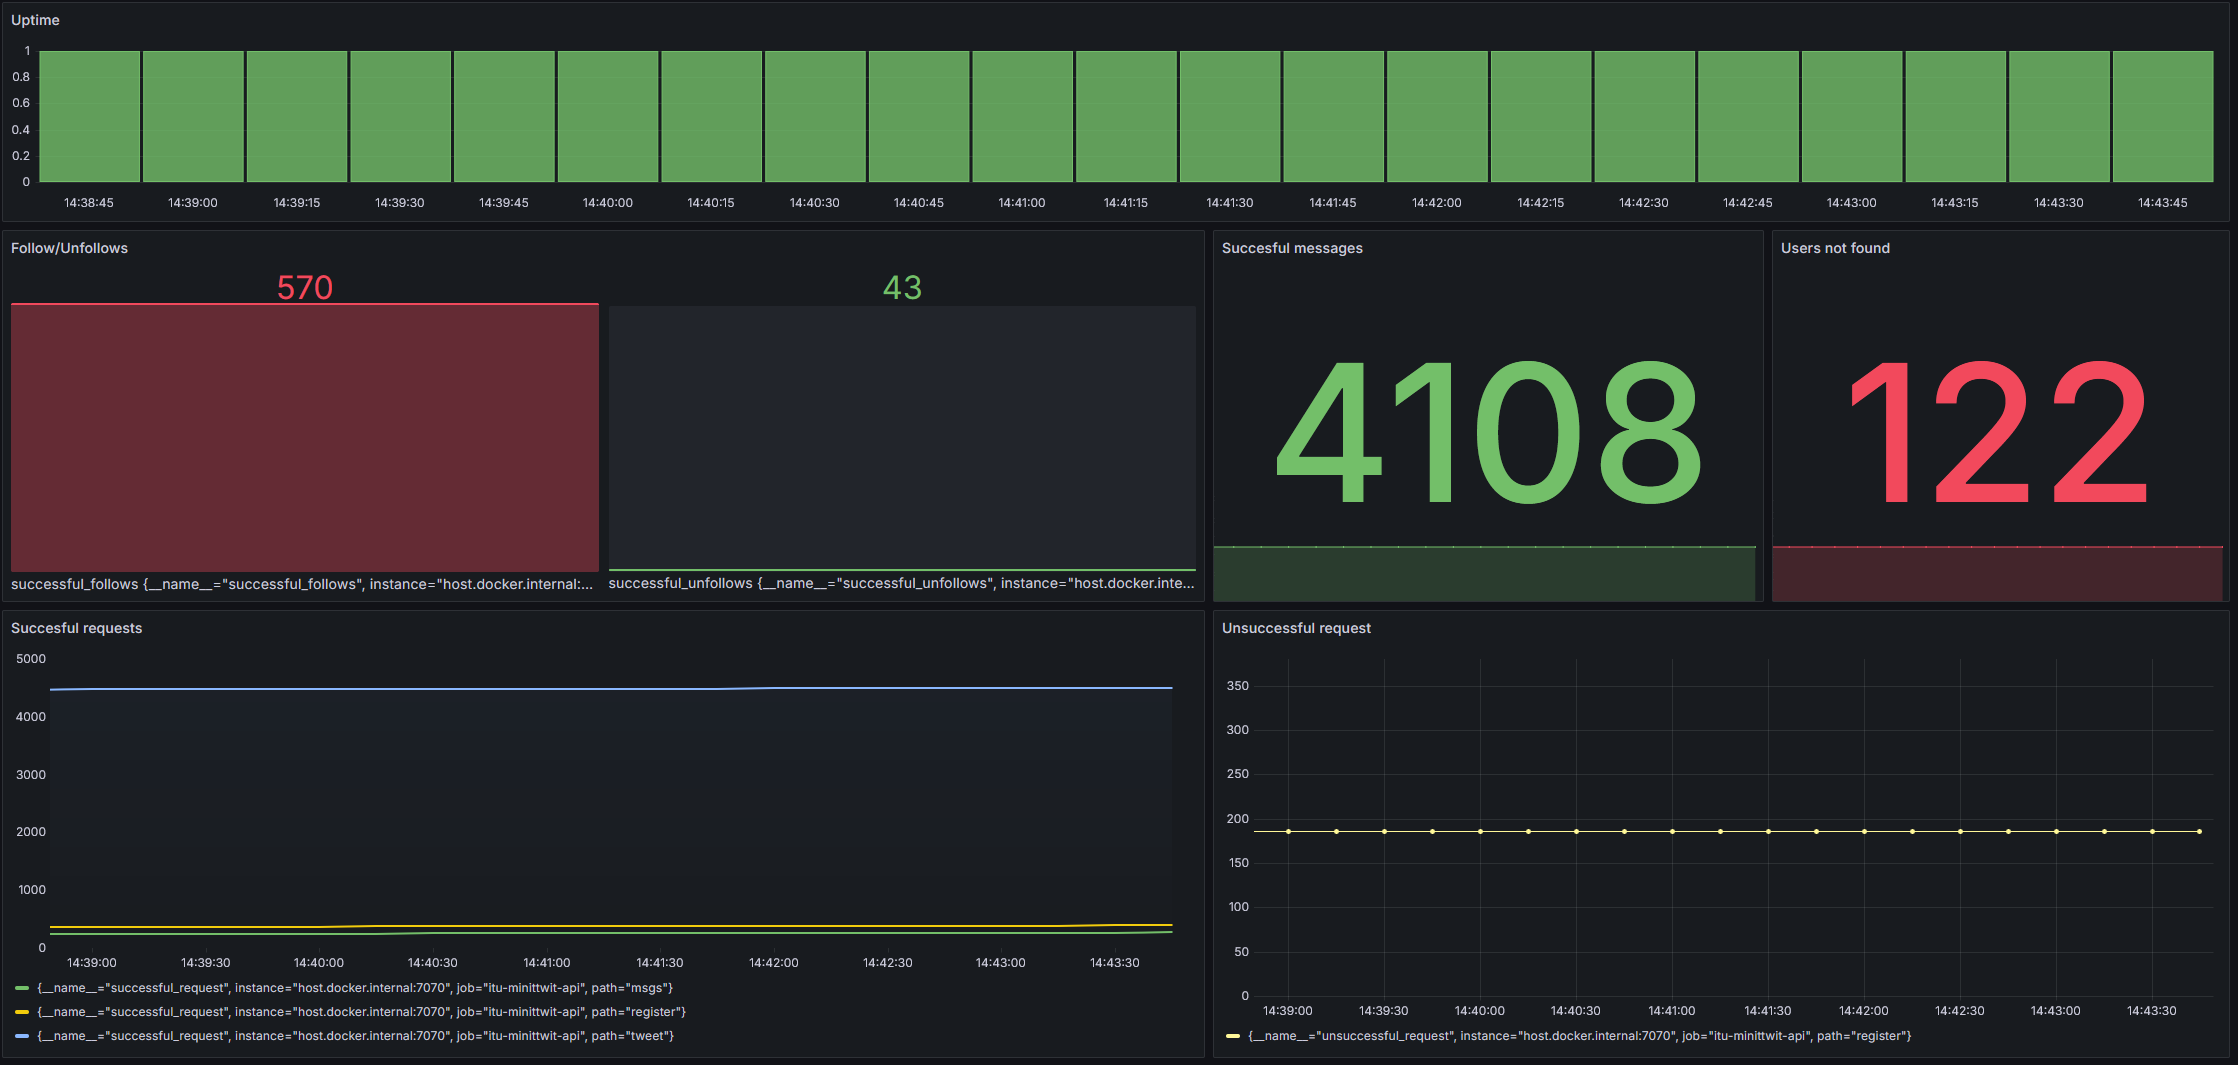
\includegraphics[width=1.0\linewidth]{Images/Grafana_dashboard.png}
    \caption{Screenshot of the Grafana dashboard showing API monitoring metrics}
    \label{fig:dashboard}
\end{figure}

\subsection{Logging}
\label{sec:logging}
To get the right logs from our system, we used a package called Logrus, which gave us full control over what we wanted to log. By setting the logging level (currently WarnLevel) and using function-level flags we avoided unnecessary verbosity. Since the system handles considerable traffic we deliberately avoided logging every event by placing a 2 second execution threshold, to help us focus on performance bottlenecks. We are mindful of not logging any sensitive information such as user credentials, tokens or personal data to ensure compliance with security best practices. However, there is no formal log rotation or retention strategy in place yet, which is something we would need to address as the system scales.\\\\
To aggregate logs, we use the ELK Stack. Filebeat collects logs from the Docker containers, and sends these on to Logstash where they are parsed and enriched. Then they are sent to Elasticsearch, which indexes them for efficient querying. Finally, we use Kibana to visualize and analyze the logs through dashboards and search interfaces. This centralized log aggregation gives us access to real-time insight into our distributed application.
%MAX
%What do you log in your systems and how do you aggregate logs?
%make a diagram of the logging stack!

\begin{figure} [!htb]
    \centering
    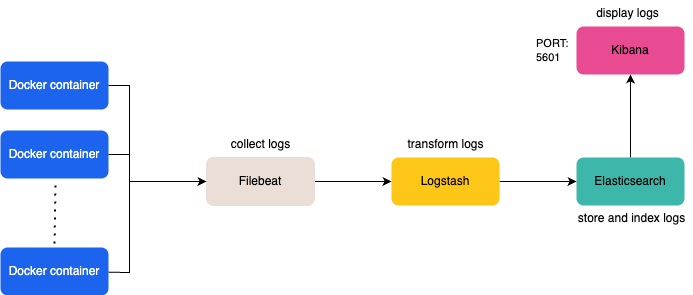
\includegraphics[width=1.0\linewidth]{Images/ELK_diagram.drawio.png}
    \caption{ELK stack used for logging}
    \label{fig:dashboard}
\end{figure}


\subsection{Security Assessment}
%gwen
%Brief results of the security assessment and brief description of how did you harden the security of your system based on the analysis.
Our security assessment revealed threats across various parts of our system. Assets at risk are listed below, along with risk scenarios and how to mitigate them:    
\begin{itemize}
    \item \textbf{Web Application} - An attacker performs SQL injection to extract sensitive user data. This is already mitigated by using ORM methods. A further step would be to automate back-ups of the database.
    
    \item \textbf{Database} - An attacker scraps Github for exposed ports, holding our database for ransom. Again, we should back up the database regularly. Configure firewalls for all droplets and update Docker Compose files.
     
    \item \textbf{API} - An attacker overwhelms the network, causing it to go down. We could avoid this by using Distributed Denial-of-Service (DDOS) protection tools which detect artificial traffic.

    \item \textbf{Github Repository} - Attacker hacks member account and steals Github secrets, exposing all other assets. In general, vulnerable passwords should be strengthened and two-factor authentication (2FA) set up.
    
    \item \textbf{Server} - An intruder gains remote access to the server via SSH, compromising the service. This is partially mitigated as we use GitHub secrets and avoid accidental exposure, however we should ensure all members have 2FA.
    
    \item \textbf{Logs} - If important events (internal or attack) are not logged properly they cannot be traced or followed up. We do already log a lot of errors however there is room for optimisation.

    \item \textbf{Monitoring} - Suspicious activity occurs however the team is not notified resulting in long response times. Ideally, our Grafana dashboard is populated with crucial metrics, e.g. number of requests per sec, and Grafana alerts are activated.

    \item \textbf{Data in Transit} - Internal communications are intercepted by malicious actors, exposing sensitive information. A Transport Layer Security (TLS) is needed to authenticate our servers and encrypt data in transit. 

    \item \textbf{Source Code} - Dependencies get outdated; updates may be incompatible and affect functionality of app. These bugs can be exploited by attackers. We could use tools such as Dependabot to keep our systems up-to-date.

\end{itemize}

The following risk matrix reflects which threats are most important to focus on. We have attempted to address the exposed ports however due to time constraints we have not yet tested the solution on Digital Ocean. Ideally, we would also integrate Dependabot, optimise monitoring metrics, use TLS, configure firewalls and automate back-ups of our database as soon as possible.

\begin{figure} [!htb]
    \centering
    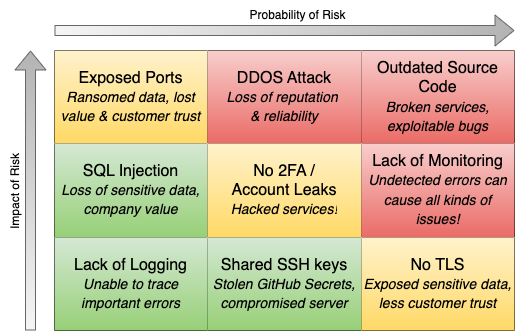
\includegraphics[width=0.7\linewidth]{Images/riskmatrix.png}
    \caption{A risk matrix which takes into account current state of system and mitigations (if any).}
    \label{fig:Seq}
\end{figure}


\subsection{Scaling and Upgrade Strategies}
%Applied strategy for scaling.
%iulia
%A complete description of the failover strategy using hot and standby server and keepalived and update strategy using green blue deployment and the floating ips

\subsubsection{High Availability via Hot-Standby Setup}

To enhance the availability and resilience of our application, we implemented a \textbf{hot-standby server setup} instead of using a container orchestration system like Docker Swarm. In this architecture:
\begin{itemize}
  \item Only one droplet is active at a time, handling all traffic.
  \item A second droplet is in standby mode, kept in sync and ready to take over instantly if the active one fails.
  \item A DigitalOcean floating IP is used to route traffic to the active server and is automatically reassigned during failover.
\end{itemize}

\subsubsection*{Implementation Steps}
We followed these steps to implement the hot-standby architecture:
\begin{itemize}
  \item Created a snapshot of the initial (active) droplet and used it to spawn the standby server.
  \item Assigned a floating IP to the active droplet.
 \item Installed and configured Keepalived on both droplets:
    \begin{itemize}
      \item \texttt{check-api.sh} monitors the health of the application.
      \item \texttt{master.sh} reassigns the floating IP upon failure detection.
      \item \texttt{keepalived.conf} and \texttt{keepalived.service} manage and start the Keepalived daemon.
    \end{itemize}
  \item Added necessary firewall rules and database access permissions on DigitalOcean.
\end{itemize}

\subsubsection*{Why We Chose Hot-Standby over Docker Swarm}
\begin{itemize}
  \item \textbf{Simplicity}: Swarm introduces added complexity and overhead in managing a cluster, which was not justified for our relatively simple application architecture.
  \item \textbf{Predictable failover behavior}: With hot-standby, only one server is live at a time, making debugging and maintenance easier.
  \item \textbf{More control over failover}: The Keepalived setup gives us full control over the logic that triggers failover.
\end{itemize}

\noindent While our hot-standby setup improves availability, it does not horizontally scale the API, meaning only one server handles traffic at a time. However, we opted for vertical scaling by upsizing both droplets and the database to better handle increased load, which we found sufficient for our current scope. If the system was under higher demand, we could have implemented horizontal scaling by running multiple active API replicas behind a load balancer or using a Docker Swarm cluster with service replicas and built-in load distribution.

\subsubsection{Blue-Green Deployment Strategy}

To handle zero-downtime updates and safe rollbacks, we implemented a Blue-Green Deployment Strategy, building on the infrastructure we already had for scaling. 

\noindent We assigned a second floating IP to the standby (passive) droplet. This enabled our CI/CD pipeline to:
\begin{enumerate}
  \item Deploy the new version of the application to the passive server (Blue).
  \item Swap the floating IPs using the DigitalOcean API after a successful deployment, making Blue the new active server (Green).
  \item Redeploy to the now-passive (previously active) server to bring both environments in sync.
\end{enumerate}

\noindent This strategy ensures that:
\begin{itemize}
  \item Deployments are atomic and safe: if the Blue deployment fails, Green remains untouched and continues serving traffic.
  \item Traffic is only routed to stable, verified servers, avoiding mid-deploy errors.
  \item Rollbacks are simple: just reverse the IP swap.
\end{itemize}

\subsubsection*{Why We Chose Blue-Green over Rolling Updates}
\begin{itemize}
  \item \textbf{Minimal complexity}: Our infrastructure is not container-orchestrated, so rolling updates would be harder to coordinate reliably.
  \item \textbf{Clear separation} between active and staging environments.
  \item \textbf{Natural fit with hot-standby}: Using floating IPs made Blue-Green deployment easy to implement with our existing failover setup.
\end{itemize}



%\clearpage
\section{Reflections}
%Describe the biggest issues, how you solved them, and which are major lessons learned.
%Link back to respective commit messages, issues, tickets, etc. to illustrate these.

\subsection{Evolution \& Refactoring}
% - Tore's big refactoring that we almost lost!
% - Long and winding road of ORM. researching properly if we actually want it, be prepared to take another road to save development cost
% - A better overview of the entire system we wanted to build would have informed some crucial decisions and saved us pain/time/both 
\begin{itemize} 
    \item Migrating from SQLite to PostgreSQL introduced several compatibility and configuration challenges, particularly around data types, secure connectivity, and credential management, all of which required adjustments in both infrastructure setup and application code.
    \item Investigating tasks thoroughly before starting them is crucial. For example, introducing GORM to our application was a long and tedious process which should have been better explored beforehand. In general, a complete overview over the entire system we were building would have informed some crucial decisions and saved us pain/time/both - we now understand why time is well spent on designing a system before building it.
    \item Refactoring should be broken down into tidbits and tackled in iterations. Also, Github best practices should not be taken for granted as common knowledge. A large refactoring of the code base was committed and pushed one night, and following day a direct merge into the main branch happened accidentally. It was time-consuming and stressful to fix, but we managed!  
\end{itemize}

\subsection{Operations}
% - logging
% - setting up keepalived 
% - writing useful error messages
\begin{itemize}
    \item After migrating to PostgreSQL, our API suddenly stopped connecting to the database. We discovered this was due to too many open connections — each request was opening a new connection. The solution was to refactor the API to use a single persistent database connection instead of reconnecting per request.
    \item Storage limitations on the remote server highlighted the need to avoid storing data inside containers and to use external volumes for persistence. To solve these issues, we also scaled vertically by increasing the size of both the droplet and the database instance.
    \item Although the group was quite good at checking the status of our system manually (very not-DevOps like), occasionally the system went down for an extended period of time without anyone noticing. It turned out that we were not monitoring the most useful metrics nor setting alerts for them; at the same time, we found our logging stack challenging to work with. We learned that familiarity with both and quick implementation of missing metrics can go a long way.
\end{itemize}

\subsection{Maintenance}

\begin{itemize}
    \item We had to update Dockerfiles and Docker Compose paths when switching to pulling images from Docker Hub. SSH command chaining required extra care due to syntax differences, and .bash profile needed to be sourced manually to ensure environment variables were available during remote setup and deployment.
    \item We learned that budget constraints can introduce challenges to maintaining the system as demand grows, but it can also scope or simplify decision-making when so many solutions (e.g. CPU type, RAM size, etc) are available. 
\end{itemize}

\subsection{On Using Large Language Models}

The team is comprised of people with a wide range of experience; some preferred using LLMs better than others. Those who used LLMs mainly used Gemini and ChatGPT to help bridge knowledge gaps in various areas of the course which were new to some if not all of us. This was especially helpful due to the high pace of the course and conflicting schedules, allowing us to maintain momentum and collaborate better. In addition, Gemini was useful as a steady hand during Git merges gone wrong and doomloop rebasing. That being said, we also experienced the negative effect LLMs can have on the development process. In particular, using LLMs heavily to assist in the ORM transition lend to more time spent on debugging and merging code. This process exposed how important it is to understand fundamentals of the code base before relying on LLMs, especially when it comes to testing functions during web development. It is clear sometimes LLMs are not suitable replacements for knowledge sharing within the team. 

%briefly explain which AI-assistants/system(s) you used during the project and reflect how it supported or hindered your process.

\subsection{On Ways of Working}
%Also reflect and describe what was the "DevOps" style of your work. For example, what did you do differently to previous development projects and how did it work?

Compared to previous projects, our team adopted a clear DevOps style by automating the entire build–test–deploy cycle through CI/CD pipelines, managing infrastructure with code, working with Github Issues and monitoring the system in production. We focused on fast feedback through automated testing and logging, which helped us catch and resolve issues early. This approach made our workflow more efficient, reliable and aligned with real-world DevOps practices. 

Given that most aspects of this project were new to us, we worked fairly smoothly as a team. We shared decision-making well, did our best to split tasks fairly, and managed expectation well according to ability and time available. The main challenge was plugging knowledge gaps in a fast-moving project while juggling other coursework. Time constraints and shifting priorities are the enemy of DevOps - it is ideal that team members are not spread over too many projects, and that there is dedicated space for knowledge sharing and hand-offs. 

%it would have been good to use developer logs! 
%bibliography 
\printbibliography
%\begin{appendices}
%\section{Appendix}

%\end{appendices}
\end{document}